
% Spellcheck: ok
% Mikes: ok

% ============================================================
\chapter{Guesstimation and the Back of~the~Envelope}{}{}
\label{ch:guesstimation}
  
\index{data analysis!guesstimation|(}
\index{guesstimation|(}
    
\Fint{Look around the room you are sitting in as you read this. Now answer
the following question:} how many Ping-Pong balls would it take to fill
this room?
    
Yes, I know it's lame to make the reader do jot'em-dot'em exercises,
and the question is old anyway, but please make the effort to come up
with a number. I am trying to make a point here.
    
Done? Good---then, tell me, what is the margin of error in your
result? How many balls, plus or minus, do you think the room might
accommodate as well? Again, numbers, please! Look at the margin of
error: can you justify it, or did you just pull some numbers out of
thin air to get me off your back? And if you found an argument to base
your estimate on: does the result seem right to you? Too large, too
small?
    
Finally, can you state the assumptions you made when answering the
first two questions? What did or did you not take into account? Did
you take the furniture out or not? Did you look up the size of a
Ping-Pong ball, or did you guess it? Did you take into account
different ways to pack spheres? Which of these assumptions has the
largest effect on the result? Continue on a second sheet of paper if
you need more space for your answer.

The game we just played is sometimes called \emph{guesstimation} and
is a close relative to the \emph{back-of-the-envelope calculation}.\index{back-of-the-envelope calculations}
The difference is minor: the way I see it, in guesstimation we worry
primarily about finding suitable input values, whereas in a typical
back-of-the-envelope calculation, the inputs are reasonably well known
and the challenge is to simplify the actual calculation to the point
that it can be done on the back of the proverbial envelope.  (Some
people seem to prefer napkins to envelopes---that's the more sociable
crowd.)
    
Let me be clear about this: I consider proficiency at guesstimation
and similar techniques the absolute hallmark of the practical data
analyst---the person who goes out and solves \emph{real} problems in
the \emph{real} world. It is so powerful because it connects a
conceptual understanding (no matter how rough) with the concrete
reality of the problem domain; it leaves no place to hide.
Guesstimation also generates \emph{numbers} (not theories or models)
with their wonderful ability to cut through vague generalities and
opinion-based discussions.
    
For all these reasons, guesstimation is a crucial skill.  It is where
the rubber meets the road.
   
The whole point of guesstimation is to come up with an approximate
answer---quickly and easily. The flip side of this is that it forces
us to think about the accuracy of the result: first how to estimate
the accuracy and then how to communicate it. That will be the program
for this chapter.

% ============================================================
\section{Principles of Guesstimation}

\index{guesstimation!principles|(}
   
Let's step through our introductory Ping-Pong ball example together.
This will give me an opportunity to point out a few techniques that
are generally useful.
    
First consider the room. It is basically rectangular in shape. I have
bookshelves along several walls; this helps me estimate the length of
each wall, since I know that shelves are 90 cm (3 ft) wide---that's a
pretty universal standard. I also know that I am 1.80 m (6 ft) tall,
which helps me estimate the height of the room. All told, this comes
to 5 m by 3.5 m by 2.5 m or about $50\text{ m}^3$.
    
Now, the Ping-Pong ball. I haven't had one in my hands for a long
time, but I seem to remember that they are about 2.5 cm (1 in) in
diameter. That means I can line up 40 of them in a meter, which means
I have $40^3$ in a cubic meter. The way I calculate this is: $40^3 =
4^3 \cdot 10^3 = 2^6 \cdot \hbox{1,000} = \text{64,000}$. That's the number of Ping-Pong balls that fit
into a cubic meter.
    
Taking things together, I can fit $50 \cdot \text{64,000}$ or
approximately 3,000,000 Ping-Pong balls into this room. That's a large
number.  If each ball costs me a dollar at a sporting goods store,
then the value of all the balls required to fill this room would be
many times greater than the value of the entire house!
    
Next, the margins of error. The uncertainty in each dimension is at
least 10 percent. Relative errors are added to each other in a
multiplication (we will discuss error propagation later in this
chapter), so the total error turns out to be $3 \cdot 10$ percent = 30
percent!  That's pretty large---the number of balls required might be
as low as two million or as high as four million. It is uncomfortable
to see how the rather harmless-looking 10 percent error in each
individual dimension has compounded to lead to a 30 percent
uncertainty.

The same problem applies to the diameter of the Ping-Pong balls.
Maybe 2.5 cm is a bit low---perhaps 3 cm is more like it. Now, that's
a 20 percent increase, which means that the number of balls fitting
into one cubic meter is reduced by 60 percent (3 times the relative
error, again): now we can fit only about 30,000 of them into a cubic
meter.  The same goes for the overall estimate: a decrease by half if
balls are 5 mm larger than initially assumed. Now the range is
something between one and two million.

Finally, the assumptions. Yes, I took the furniture out. Given the
uncertainty in the total volume of the room, the space taken up by the
furniture does not matter much. I also assumed that balls would stack
like cubes, when in reality they pack tighter if we arrange them in
the way oranges (or cannonballs) are stacked. It's a slightly
nontrivial exercise in geometry to work out the factor, but it comes
to about 15 percent more balls in the same space.
    
So, what can we now say with certainty? We will need a few million
Ping-Pong balls---probably not less than one million and certainly not
more than five million. The biggest uncertainty is the size of the
balls themselves; if we need a more accurate estimate than the one
we've obtained so far, then we can look up their exact dimensions and
adjust the result accordingly.
    
(After I wrote this paragraph, I finally looked up the size of a
regulation Ping-Pong ball: 38--40 mm. Oops. This means that only about
15,000 balls fit into a cubic meter, and so I must adjust all my
estimates down by a factor of 4.)
    
This example demonstrates all important aspects of guesstimation:

\begin{itemize}
\item Estimate sizes of things by comparing them to something you
  know.
\item Establish functional relationships by using simplifying
  assumptions.
\item Originally innocuous errors can compound dramatically, so
  tracking the accuracy of an estimate is crucial.
\item And finally, a few bad guesses on things that are not very
  familiar can have a devastating effect (I really haven't played
  Ping-Pong in a long time), but they can be corrected easily when
  better input is available.
\end{itemize}
    
Still, we did find the order of magnitude, one way or the other: a few
million.

\subsection{Estimating Sizes}

\index{size, estimating} 
    
The best way to estimate the size of an object is to compare it to
something you know. The shelves played this role in the previous
example, although sometimes you have to work a little harder to find a
familiar object to use as reference in any given situation.
    
Obviously, this is easier to do the more you know, and it can be very
frustrating to find yourself in a situation\vadjust{\pagebreak} where you don't know
anything you could use as a reference. That being said, it is usually
possible to go quite far with just a few data points to use as
reference values.

(There are stories from the Middle Ages of how soldiers would count
how many rows of stone blocks were used in the walls of a fortress
before mounting an attack, the better to estimate the height of the
walls.  Obtaining an accurate value was necessary to prepare scaling
ladders of the appropriate length: if the ladders were too short, then
the top of the wall could not be reached; if they were too long, the
defenders could grab the overhanging tops and topple the ladders back
over. Bottom line: you've got to find your reference objects where you
can.)
    
Knowing the sizes of things is therefore the first order of business.
The more you know, the easier it is to form an estimate; but also the
more you know, the more you develop a feeling for the correct answer.
That is an important step when operating with guesstimates: to perform
an independent ``sanity check'' at the end to ensure we did not make
some horrible mistake along the way.  (In fact, the general advice is
that ``two (independent) estimates are better than one''; this is
certainly true but not always possible---at least I can't think of an
independent way to work out the Ping-Pong ball example we started
with.)
    
Knowing the sizes of things can be \emph{learned}. All it takes is a
healthy interest in the world around you---please don't go through the
dictionary, memorizing data points in alphabetical order.  This is not
about beating your buddies at a game of Trivial Pursuit!  Instead,
this is about becoming familiar (I'd almost say intimate) with the
world you live in.  Feynman once wrote about Hans A.\ Bethe that
``every number was near something he knew.'' That is the ideal.
% Certainly you are joking, p175 
   
The next step is to \emph{look things up}. \index{lookup tables, estimating sizes} In situations where one
frequently needs relatively good approximations to problems coming
from a comparably small problem domain, special-purpose lookup tables
can be a great help. I vividly remember a situation in a senior
physics lab where we were working on an experiment (I believe, to
measure the muon lifetime), when the instructor came by and asked us
some guesstimation problem---I forget what it was, but it was
nontrivial. None of us had a clue, so he whipped out from his back
pocket a small booklet the size of a playing card that listed the
physical properties of all kinds of subnuclear particles. For almost
any situation that could arise in the lab, he had an approximate
answer right there.
    
Specialized lookup tables exist in all kinds of disciplines, and you
might want to make your own as necessary for whatever it is you are
working on. The funniest I have seen gave typical sizes (and costs)
for all elements of a manufacturing plant or warehouse: so many square
feet for the office of the general manager, so many square feet for
his assistant (half the size of the boss's), down to the number of
square feet per toilet stall, and---not to forget---how many toilets
to budget for every 20 workers per 8-hour shift.

Finally, if we don't know anything close and we can't look anything
up, then we can try to estimate ``from the ground\vadjust{\pagebreak} up'': starting just
with what we know and then piling up arguments to arrive at an
estimate. The problem with this approach is that the result may be
\emph{way} off. We have seen earlier how errors compound, and the
more steps we have in our line of arguments the larger the final error
is likely to be---possibly becoming so large that the result will be
useless. If that's the case, we can still try and find a cleverer
argument that makes do with fewer argument steps. But I have to
acknowledge that occasionally we will find ourselves simply stuck:
unable to make an adequate estimate with the information we have.
    
The trick is to make sure this happens only rarely.

\subsection{Establishing Relationships}

\index{relationships, establishing} 
     
Establishing relationships that get us from what we know to what we
want to find is usually not that hard.  This is true in particular
under common business scenarios, where the questions often revolve
around rather simple relationships (how something fits into something
else, how many items of a kind there are, and the like). In scientific
applications, this type of argument can be harder. But for most
situations that we are likely to encounter outside the science lab,
simple geometric and counting arguments will suffice.
    
In the next chapter, we will discuss in more detail the kinds of
arguments you can use to establish relationships. For now, just one
recommendation: \emph{make} it simple! Not: \emph{keep} it simple
because, more likely than not, initially the problem is \emph{not}
simple; hence you have to make it so in order to make it tractable.
    
Simplifying assumptions let you cut through the fog and get to the
essentials of a situation. You may incur an error as you simplify the
problem, and you will want to estimate its effect, but at least you are
moving toward a result.

An anecdote illustrates what I mean. When working for Amazon.com, I
had a discussion with  a rather sophisticated mathematician about how
many packages Amazon can typically fit onto a tractor-trailer truck,
and he started to work out the different ways you can \emph{stack}
rectangular boxes into the back of the truck! This is entirely missing
the point because, for a rough calculation, we can make the
simplifying assumption that the packages can take any shape at all
(\ie, they behave like a liquid) and simply divide the total volume of
the truck by the typical volume of a package. Since the individual
package is tiny compared to the size of the truck, the specific shapes
and arrangements of individual packages are irrelevant: their effect
is much smaller than the errors in our estimates for the size of the
truck, for instance. (We'll discuss this in more detail in Chapter
\ref{ch:scaling}, where we discuss the mean-field approximation.)

The point of back-of-the-envelope estimates is to retain only the core
of the problem, stripping away as much nonessential detail as
possible. Be careful that your sophistication does not get in the way
of finding simple answers.

\subsection{Working with Numbers}
  
When working with numbers, don't automatically reach for a calculator!
I know that I am now running the risk of sounding ridiculous---praising
the virtues of old-fashioned reading, 'riting, and 'rithmetic. But
that's not my point. My point is that it is \emph{all right} to work
with numbers. There is no reason to avoid them.
    
I have seen the following scenario occur countless times: a discussion
is under way, everyone is involved, ideas are flying, concentration is
intense---when all of a sudden we need a few numbers to proceed.
Immediately, \emph{everything} comes to a screeching halt while
several people grope for their calculators and others fire up their
computers, followed by hasty attempts to get the required answer,
which invariably (given the haste) leads to numerous keying errors and
false starts, followed by arguments about the best calculator software
to use. In any case, the whole creative process just died. It's a
shame.
    
Besides forcing you to switch context, calculators remove you one step
further from the nature of the problem. When working out a problem in
your head, you get a feeling for the significant digits in the result:
for which digits does the result change as the inputs take on any
value from their permissible range? The surest sign that somebody has
no clue is when they quote the results from a calculation based on
order-of-magnitude inputs to 16 digits!
    
The whole point here is not to be religious about it---either way.  If
it actually becomes more complicated to work out a numerical
approximation in your head, then by all means use a calculator.  But
the compulsive habit to avoid working with numbers at all cost should
be restrained.
    
There are a few good techniques that help with the kinds of
calculations required for back-of-the-envelope estimates and that are
simple enough that they still (even today) hold their own against
uncritical calculator use. Only the first is a must-have; the other
two are optional.

\subsubsection{Powers of ten}

\index{powers of ten} 

The most important technique for deriving order-of-magnitude \index{order-of-magnitude estimates} estimates
is to work with orders of magnitudes directly---that is, with powers of
ten.
    
It quickly gets confusing to multiply 9,000 by 17 and then to divide
by 400, and so on. Instead of trying to work with the numbers
directly, split each number into the most significant digit (or
digits) and the respective power of ten. The multiplications now take
place among the digits only while the powers of ten are summed up
separately. In the example I just gave, we split $\text{9,000} = 9
\cdot \text{1,000}$, $17 = 1.7 \cdot 10 \approx 2 \cdot 10$, and $400
= 4 \cdot 100$.  From the leading digits we have $9$ times $2$ divided
by $4$ equals $4.5$, and from the powers of ten we have $3$ plus $1$
minus $2$ equals $2$; so then $4.5 \cdot 10^2 = 450$.  That wasn't so
hard, was it? (I have replaced 17 with $2 \cdot 10$ in this
approximation, so\vadjust{\pagebreak} the result is a bit on the high side, by about 15
percent. I might want to correct for that in the end---a better
approximation would be closer to $390$. The exact value is $382.5$.)
    
More systematically, any number can be split into a decimal fraction
and a power of ten. It will be most convenient to require the fraction
to have exactly one digit before the decimal point, like so:
\begin{gather*}
123.45 = 1.2345 \cdot 10^2 \\
\text{1,000,000} = 1.0 \cdot 10^6 \\
0.00321 = 3.21 \cdot 10^{-3}
\end{gather*}   
    
The fraction is commonly known as the \emph{mantissa} (or the
\emph{significand} in most recent usage), whereas the power of ten is
always referred to as the \emph{exponent}.
    
This notation significantly simplifies multiplication and division
between numbers of very different magnitude: the mantissas multiply
(involving only single-digit multiplications, if we restrict ourselves
to the most significant digit), and the exponents add. The biggest
challenge is to keep the two different tallies simultaneously in one's
head.

\subsubsection{Small perturbations}
    
\index{perturbation theory}     
    
The techniques in this section are part of a much larger family of
methods known as \emph{perturbation theory}, methods that play a huge
role in applied mathematics and related fields. The idea is always the
same---we split the original problem into two parts: one that is easy
to solve and one that is somehow ``small'' compared to the first. If
we do it right, the effect of the latter part is only a ``small
perturbation'' to the first, easy part of the problem. (You may want
to review Appendix \ref{app:calculus} if some of this material is
unfamiliar to you.)
    
The easiest application of this idea is in the calculation of simple
powers, such as $12^3$. Here is how we would proceed:
\begin{align*}
12^3 = (10+2)^3 & = 10^3 + 3 \cdot 10^2 \cdot 2 
                         + 3 \cdot 10 \cdot 2^2 + 2^3 \\
                & = \text{1,000} + 600 + \dotsb \\
                & = \text{1,600} + \dotsb
\end{align*}
    
In the first step, we split $12$ into $10 + 2$: here $10$ is the easy
part (because we know how to raise $10$ to an integer power) and $2$
is the perturbation (because $2 \ll 10$).  In the next step, we make
use of the binomial formula (see Appendix \ref{app:calculus}),
ignoring everything except the linear term in the ``perturbation.''
The final result is pretty close to the exact value.
    
The same principle can be applied to many other situations.  In the
context of this chapter, I am interested in this concept because  it
gives us a way to estimate and correct for the error introduced by
ignoring all but the first digit in powers-of-ten calculations.  Let's
look at another example:
%
\[
32 \cdot 430
\]
%
Using only the most significant digits, this is $(3 \cdot 10^1) \cdot
(4 \cdot 10^2) = (3 \cdot 4) \cdot 10^{1 + 2} = \text{12,000}$. But
this is clearly not correct, because we dropped some digits from the
factors.

We can consider the nonleading digits as \emph{small perturbations} to
the result and treat them separately. In other words, the calculation
becomes:
% 
\[ (3 + 0.2) \cdot (4 + 0.3) \cdot 10^3 
\approx 3 (1 + 0.1\dotsc) \cdot 4 (1+0.1\dotsc) \cdot 10^3 
\] 
% 
where I have \emph{factored out} the largest factor in each term. On
the righthand side I did not write out the correction terms in
full---for our purposes, it's enough to know that they are about $0.1$.
    
%We can consider the nonleading digits as \emph{small perturbations} to
%the result and treat them separately. In other words, the calculation
%becomes $(3 + 0.2) \cdot (4 + 0.3) \approx 3 (1 + 0.1\dotsc) \cdot\break 4
%(1+0.1\dotsc)$, where I have \emph{factored out} the largest factor in
%each term. On the righthand side I did not write out the correction
%terms in full---for our purposes, it's enough to know that they are
%about $0.1$.
    
Now we can make use of the binomial formula:
%
\[
(1 + \epsilon)^2 = 1 + 2 \epsilon + \epsilon^2
\]
%
We drop the last term (since it will be very small compared to the
other two), but the second term gives us the size of the correction:
$+ 2 \epsilon$. In our case, this amounts to about 20 percent, since
$\epsilon$ is one tenth.
    
I will admit that this technique seems somewhat out of place today,
although I do use it for real calculations when I don't have a
calculator on me. But the true value of this method is that it enables
me to estimate and reason about the effect that changes to my input
variables will have on the overall outcome. In other words, this
method is a first step toward \emph{sensitivity analysis}.\index{sensitivity analysis, perturbation theory}

\subsubsection{Logarithms}

\index{logarithms!about}
 
This is the method by which generations before us performed numerical
calculations. The crucial insight is that we can use logarithms for
products (and exponentiation) by making use of the functional equation
for logarithms:
%
\[
\log( x y ) = \log(x) + \log(y)
\]
%
In other words, instead of \emph{multiplying} two numbers, we can
\emph{add} their logarithms. The slide rule was a mechanical
calculator based on this idea.
    
Amazingly, using logarithms for multiplication is \emph{still}
relevant---but in a slightly different context. For many statistical
applications (in particular when using Bayesian methods), we need to
multiply the probabilities of individual events in order to arrive at
the probability for the combination of these events. Since
probabilities are by construction less than $1$, the product of any
two probabilities is always smaller than the individual factors. It
does not take many probability factors to underflow the floating-point
precision of almost any standard computer. Logarithms to the rescue!
Instead of multiplying the probabilities, take logarithms of the
individual probabilities and then add the logarithms.  (The logarithm
of a number that is less than $1$ is negative, so one usually works
with $-\log(p)$.)  The resulting numbers, although mathematically
equivalent, have much better numerical properties. Finally, since in
many applications we\vadjust{\pagebreak} mostly care which of a selection of different
events has the maximum probability, we don't even need to convert back
to probabilities: the event with maximum probability will also be the
one with the maximum (negative) logarithm.

\subsection{More Examples}

We have all seen this scene in many a Hollywood movie: the gangster
comes in to pay off the hitman (or pay for the drug deal, or whatever
it is). Invariably, he hands over an elegant briefcase with the
money---cash, obviously. Question: how much is in the case?

Well, a briefcase is usually sized to hold two letter-size papers next
to each other; hence it is about 17 by 11 inches wide, and maybe 3
inches tall (or 40 by 30 by 7 centimeters). A bank note is about 6
inches wide and 3 inches tall, which means that we can fit about six
per sheet of paper. Finally, a 500-page ream of printer paper is about
2 inches thick.  All told, we end up with $2 \cdot 6 \cdot 750 =
\text{9,000}$ banknotes.  The highest dollar denomination in general
circulation is the \$100 bill,\footnote{Larger denominations exist
  but---although legal tender---are not officially in circulation and
  apparently fetch far more than their face value among collectors.} 
so the maximum value of that payoff was about \$1 million, and
certainly not more than \$5 million.

Conclusion: for the really big jobs, you need to pay by check. Or use
direct transfer.

For a completely different example, consider the following question.
What's the typical takeoff weight of a large, intercontinental jet
airplane? It turns out that you can come up with an approximate answer 
even if you don't know \emph{anything} about planes. 

A plane is basically an aluminum tube with wings. Ignore the wings for
now; let's concentrate on the tube. How big is it? One way to find out
is to check your boarding pass: it will display your row number.
Unless you are much classier than your author, chances are that it
shows a row number in the range of 40--50. You can estimate that the
distance between seats is a bit over $50 \text{ cm}$---although it
feels closer. (When you stand in the aisle, facing sideways, you can
place both hands comfortably on the tops of two consecutive seats;
your shoulders are about $30$ cm apart, so the distance between seats
must be a tad greater than that.) Thus we have the length: $50 \cdot
0.5\text{ m}$. We double this to make up for first and business class,
and to account for cockpit and tail.  Therefore, the length of the
tube is about $50 \text{ m}$. How about its diameter? Back in economy,
rows are about $9$ seats abreast, plus two  aisles. Each seat being
just a bit wider than your shoulders (hopefully), we end up with a
diameter of about $5 \text{ m}$.  Hence we are dealing with a tube
that is $50 \text{ m}$ long and $5 \text{ m}$ in diameter.

As you walked through the door, you might have noticed the strength or
thickness of the tube: it's about $5 \text{ mm}$. Let's make that $10
\text{ mm}$ ($1 \text{ cm}$) to account for ``stuff'': wiring, seats,
and all kinds of other hardware that's in the plane. Imagining now
that you unroll the entire plane (the way you unroll\vadjust{\pagebreak} aluminum foil),
the result is a sheet that is $50 \cdot \pi \cdot 5 \cdot 0.0 1
\text{m}^3$. The density of aluminum is a little higher than water (if you
have ever been to a country that uses aluminum coins, you know that you can barely make them float), so let's say it's $3 \text{ g}/\text{cm}^3$.

It is at this point that we need to employ the proverbial back of the
envelope \index{back-of-the-envelope calculations} (or the cocktail napkin they gave you with the peanuts) to
work out the numbers. It will help to realize that there are $100^3 =
10^6$ cubic centimeters in a cubic meter and that the density 
of~aluminum can therefore be written as $3$ tons per cubic meter. The
final mass of the ``tube'' comes out to about $25$ ton. Let's double
this to take into account the wings (wings are about as long as the
fuselage is wide---if you look at the silhouette of a plane in the
sky,~it forms an approximate square); this yields $50$ ton just for
the ``shell'' of the airplane. It does not take into account the
engines and most of the other equipment inside the plane.

Now let's compare this number with the load. We have $50$ rows, half
of them with 9 passengers and the other half with 5; this gives
us an average of 7 passengers per row or a total of $350$
passengers per plane. Assuming that each passenger contributes $100
\text{ kg}$ (body weight and baggage), the load amounts to $35$ ton:
comparable to the weight of the plane itself. (This weight-to-load
ratio is actually not that different than for a car, fully occupied by
four people. Of course, if you are driving alone, then the ratio for
the car is \emph{much} worse.)

How well are we doing? Actually, not bad at all: Table
\ref{tbl:planes} lists typical values for three planes that are common
on transatlantic routes: the mid size Boeing 767, the large Boeing 747
(the ``Jumbo''), and the extra-large Airbus 380. That's enough to
check our calculations. We are not far off.

(What we totally missed is that planes don't fly on air and in-flight
peanuts alone: in fact, the greatest single contribution to the weight
of a fully loaded and fuelled airplane is the weight of the
\emph{fuel}. You can estimate its weight as well, but to do so, you
will need one additional bit of information: the fuel consumption of a
modern jet airplane per passenger and mile traveled is less than that
of a typical compact car with only a single passenger.)

\begin{table}
\def\a{\hphantom{.0}}
\def\b{\hphantom{0}}
\newlength{\guesslen}
\tbl{Approximate measurements for some common intercontinental jets
\label{tbl:planes}}{%
\begin{tabular}{@{\hskip6pt}ccccccc@{\hskip6pt}}
\toprule
&&& &\TCH{Weight} & \TCH{Weight}\\
 & {\TCH{Length}} & {\TCH{Width}} & {\TCH{Diameter}}
                  &                    {\TCH{(empty)}}
                   &  {\TCH{(full)}}
                  & {\TCH{Passengers}} \\\colrule
B767 & 50 m    & 50 m   & 5 m\a  &  \b90 t  & 150 t & 200  \\
B747 & 70 m    & 60 m   & 6.5 m & 175 t  & 350 t & 400 \\
A380 & 75 m    & 80 m   & 7 m\a   & 275 t  & 550 t & 500 \\
\end{tabular}}\vspace*{6pt}
\end{table}

That was a long and involved estimation, and I won't blame you if you
skipped some of the intermediate steps. In case you are just joining
us again, I'd like to emphasize one point: we came up with a
reasonable estimate without having to resort to any ``seat of the
pants'' estimates---even though we had no prior\vadjust{\pagebreak} knowledge! Everything
that we used, we could either observe directly (such as the number of
rows in the plane or the thickness of the fuselage walls) or could
relate to something that was familiar to us (such as the distance
between seats). That's an important takeaway!

But not all calculations have to be complicated. Sometimes, all you
have to do is ``put two and two together.'' A friend told me recently
that his company had to cut their budget by a million dollars. We knew
that the overall budget for this company was about five million
dollars annually. I also knew that, since it was mostly a service
company, almost all of its budget went to payroll (there was no
inventory or rent to speak of). I could therefore tell my friend that
layoffs were around the corner---even with a salary reduction program,
the company would have to cut at least 15 percent of their staff. The
response was: ``Oh, no, our management would \emph{never} do that.''
Two weeks later, the company eliminated one third of all
positions.


\subsection{Things I Know}
    
Table \ref{tbl:guesstimation} is a collection of things that I know
and frequently use to make estimates. Of course, this list
may seem a bit whimsical, but it is actually pretty serious. For
instance, note the \emph{range} of areas from which these items are
drawn! What domains can you reason about, given the information in
this table?
    
Also notice the absence of systematic ``scales.'' That is no accident.
I don't need to memorize the weights of a mouse, a cat, and a
horse---because I know (or can guess) that a mouse is 1,000 times
smaller than a human, a cat 10 times smaller, and a horse 10 times
larger. The items in this table are \emph{not} intended to be
comprehensive; in fact, they are the bare minimum. Knowing how things
relate to each other lets me take it from there.
    
Of course, this table reflects my personal history and interests.
Yours will be different.


%\setcounter{table}{1}
%\begin{table}[t!]
%\tbl{Reference points for guesstimations.}{%
%\begin{tabular}{lp{0.5\textwidth}}
%\hline
%\rule{0mm}{4mm}%
%                                      & \\
%American Civil War; Franco-Prussian War & 1860s; 1870s \\
%French Revolution			& 1789 \\
%Reformation				& 1517 \\
%Charlemagne				&  800 \\
%Great Pyramids			        & 3000 B.C.E. \\
%                                        & \\
%Hot day                                 & 35 Celsius \\
%Very hot kitchen oven		        & 250 Celsius \\
%Steel melts				& 1200 Celsius \\
%                                        & \\
%Density of water                        & $1\text{ g}/\text{cm}^3$ \\
%Density of aluminum                     & $3\text{ g}/\text{cm}^3$ \\
%Density of lead                         & $13\text{ g}/\text{cm}^3$ \\
%Density of gold                         & $20\text{ g}/\text{cm}^3$ \\
%                                        & \\
%Ionization energy of hydrogen           & 13.6 eV \\
%Atomic diameter (Bohr radius)           & $10^{-10}\text{ m}$ \\
%Energy of X-ray radiation               & keV \\
%Nuclear binding energy per particle     & MeV \\
%Sodium doublet                          & 590 nm \\
%\hline
%\end{tabular}}\vspace*{6pt}
%\end{table}

% Common simplifying assumptions:
% - All biological materials are mostly water and hence have 
%   the density of water.
% - All things are spherical or cubic
% 
% Things I don't know:
% - Daily turnover at the NYSE
% - National debt
% - Distance Earth Moon
% - Length of a trans-ocean container
% - Human energy consumption per day

\index{guesstimation!principles|)}

% ============================================================
\section{How Good Are Those Numbers?}

\index{guesstimation!numerical correctness|(} 
   
Remember the Ping-Pong ball question that started out this chapter? I
once posted that question as a homework problem in a class, and one
student's answer was something like 1,020,408.16327.  (Did you catch
\emph{both} mistakes? Not only does the result of this rough estimate
pretend to be accurate to within a single ball; but the answer also
includes a fractional part---which is meaningless, given the context.)
This type of confusion is incredibly common: we focus so much on the
calculation (any calculation) that we forget to interpret the result!

This story serves as a reminder that there are two questions that we
should ask \emph{before} any calculation as well as one 
\emph{afterward}. The two questions to ask before we begin are:
\begin{itemize}
\item What level of correctness do I \emph{need}?
\item What level of correctness can I \emph{afford}?
\end{itemize}
\clearpage

\begin{table}[t!]
%\tabcolsep9pt
\tbl{Reference points for guesstimations
\label{tbl:guesstimation}}{%
 \begin{tabular}{lp{0.5\textwidth}}\toprule
\rule{0mm}{4mm}%
Size of an atomic data type           & 10 bytes \\
A page of text                        & 55 lines of 80 characters, or about
                                        4,500 characters  total \\
A record (of anything)                & 100--1,000 bytes \\
                                      & \\[-6pt]
A car                                 & 4 m long, 1 ton weight \\
A person                              & 2 m tall, 100 kg weight \\
A shelf                               & 1 m wide, 2 m tall \\
Swimming pool (not Olympic)           & 25 $\times$ 12.5 meters \\
A story in a commercial building      & 4 m high \\
                                      & \\[-6pt]
Passengers on a large airplane        & 350 \\
Speed of a jetliner                  & 1,000 km/hr \\
Flight time from NY                   & 6 hr 
                                        (to the West Coast or Europe)\\
                                      & \\[-6pt]
Human, walking                        & 1 m/s (5 km/hr) \\
Human, maximum power output           & 200 W (not sustainable) \\
                                      & \\[-6pt]
Power consumption of a water kettle   & 2 kW \\
Electricity grid                      & 100 V (U.S.), 220 V (Europe) \\
Household fuse                        & 16 A \\
                                      & \\[-6pt]
3 $\cdot$ 3                           & 10 (minus 10\%) \\
$\pi$                                 & 3 \\
                                      & \\[-6pt]
Large city                            & 1 million \\
Population, Germany or Japan          & 100 million \\
Population, USA                       & 300 million \\
Population, China or India            & 1 billion \\
Population, Earth                     & 7 billion \\
                                      & \\[-6pt]
U.S.\ median annual income            & \$60,000 \\
U.S.\ federal income tax rate         & 25\% (but also as low as 0\%
                                              and as high as 40\%) \\
Minimum hourly wage                   & \$10 per hour \\
Billable hours in a year              & 2,000 
                                        (50 weeks at 40 hours per week) \\
Low annual inflation                  & 2\% \\
High annual inflation                 & 8\% \\
                                      & \\ [-6pt]
Price of a B-2 bomber                  & \$2 billion \\
                                      & \\[-6pt]
American Civil War; Franco-Prussian War & 1860s; 1870s \\
French Revolution			& 1789 \\
Reformation				& 1517 \\
Charlemagne				&  800 \\
Great Pyramids			        & 3000 B.C.E. \\
                                        & \\[-6pt]
Hot day                                 & 35 Celsius \\
Very hot kitchen oven		        & 250 Celsius \\
Steel melts				& 1200 Celsius \\
                                        & \\[-6pt]
Density of water                        & 1 {g}/{cm}$^3$ \\
Density of aluminum                     & 3 g/{cm}$^3$ \\
Density of lead                         & 13 {g}/{cm}$^3$ \\
Density of gold                         & 20$\text{ g}/\text{cm}^3$ \\
                                        & \\[-6pt]
Ionization energy of hydrogen           & 13.6 eV \\
Atomic diameter (Bohr radius)           & $\hbox{10}^{-\hbox{\scriptsize 10}}\text{ m}$ \\
Energy of X-ray radiation               & keV \\
Nuclear binding energy per particle     & MeV \\
Wavelength of the sodium doublet                          & 590 nm \\
\end{tabular}}
\end{table}

\clearpage
   
The question to ask afterward is:
\begin{itemize}
\item What level of correctness did I \emph{achieve}?
\end{itemize}

I use the term ``correctness'' here a bit loosely to refer to the
quality of the result. There are actually two different concepts
involved: \emph{accuracy} and \emph{precision}.
\begin{unnumlist}
\mysubparagraph{Accuracy}
\item \index{accuracy!defined} Accuracy expresses how close the result of a calculation
  or measurement comes to the ``true'' value. Low accuracy is due to
  systematic error.
\mysubparagraph{Precision} \index{precision!defined} 
\item Precision refers to the ``margin of error'' \index{margin of error} in the 
  calculation or the experiment. In experimental situations, precision
  tells us how far the results will stray when the experiment is 
  repeated several times. Low precision is due to random noise.
\end{unnumlist}

Said another way: accuracy is a measure for the correctness of the
result, and precision is a measure of the result's uncertainty.

\vspace*{-12pt}
\subsection{Before You Get Started: Feasibility and Cost}
\index{feasibility, numerical correctness}
\index{costs!numerical correctness}
     
The first question (what level of correctness is needed) will define
the overall approach---if I only need an order-of-magnitude
approximation, then the proverbial back of the envelope will do; if I
need better results, I might need to work harder. The second question
is the necessary corollary: it asks whether I will be able to achieve
my goal given the available resources. In other words, these two
questions pose a classic engineering trade-off (\ie, they require
a regular cost--benefit analysis).

\leaflong{12pt}
    
This obviously does not matter much for a throwaway calculation, but
it matters a lot for bigger projects.  I once witnessed a huge project
(involving a dozen developers for over a year) to build a computation
engine that had failed to come clear on both counts until it was too
late.  The project was eventually canceled when it turned out that it
would cost \emph{more} to achieve the accuracy required than the
project was supposed to gain the company in increased revenue! (Don't
laugh---it could happen to you.  Or at least in your company.)
    
This story points to an important fact: correctness is usually
expensive, and high correctness is often \emph{disproportionally} more
expensive.  In other words, a 20 percent approximation can be done on
the back of an envelope, a 5 percent solution can be done in a couple
of months, but the cost for a 1 percent solution may be astronomical.
It is also not uncommon that there is no middle ground (\eg, an
affordable 10 percent solution).

I have also seen the opposite problem: projects chasing correctness
that is not really necessary---or not achievable because the required
input data is not available or of poor quality. This is a particular
risk if  the project involves the opportunity to play with some
attractive new technology.
    
Finding out the true cost or benefit of higher-quality results can
often be tricky.  I was working on a project to forecast the daily
number of visitors viewing the company's website, when I was told that
``we must have absolute\vadjust{\pagebreak} forecast accuracy; nothing else matters.'' I
suggested that if this were so, then we should take the entire site
\emph{down}, since doing so would guarantee a perfect forecast (zero
page views). Yet because this would also imply zero revenue from
display advertising, my suggestion focused the client's mind
wonderfully to define more clearly what ``else'' mattered.


\subsection{After You Finish: Quoting and Displaying Numbers}
    
It is obviously pointless to report or quote results to more digits
than is warranted.  In fact, it is misleading or at the very least
unhelpful, because it fails to communicate to the reader another
important aspect of the result---namely its reliability!
    
A good rule (sometimes known as \emph{Ehrenberg's rule}) \index{Ehrenberg's rule} is to quote
all digits up to and including the \emph{first two variable digits}.
Starting from the left, you keep all digits that do not change over
the entire range of numbers from one data point to the next; then you
also keep the first two digits that vary over the \emph{entire range}
from 0 to 9 as you scan over all data points. An example will make
this clear. Consider the following data set:

\begin{verbatim}
121.733
122.129
121.492
119.782
120.890
123.129
\end{verbatim}
    
Here, the first digit (from the left) is always 1 and the second digit
takes on only two values (1 and 2), so we retain them both.  All
further digits can take on any value between 0 and 9, and we retain
the first two of them---meaning that we retain a total of \emph{four}
digits from the left.  The two right-most digits therefore carry no
significance, and we can drop them when quoting results. The mean (for
instance) should be reported as:

\begin{verbatim}
121.5
\end{verbatim}
    
Displaying further digits is of no value.\index{accuracy!displaying}
    
This rule---to retain the first two digits that vary over the entire
range of values and all digits to the left of them---works well with
the methods described in this chapter. If you are working with numbers
as I suggested earlier, then you also develop a sense for the digits
that are largely unaffected by reasonable variations in the input
parameters as well as for the position in the result after which
uncertainties in the input parameters corrupt the outcome.
    
Finally, a word of warning. The accuracy level of a numerical result
should be established from the outset, since doing so later will
trigger resistance. I have encountered a system that reported
projected sales numbers (which were typically in the hundreds of
thousands) to six ``significant'' digits (\eg, as 324,592 or so).  But
because these were forecasts that were \emph{at best} accurate to
within 30 percent,  \emph{all} digits beyond the first were absolute
junk! (Note that 30 percent\vadjust{\pagebreak} of 300,000 is 100,000, which means that
the confidence band for this result was 200,000--400,000.)  However, a
later release of the same software, which now reported only the
actually significant digits, was met by violent opposition from the
user community because it was ``so much less precise''!

\index{guesstimation!numerical correctness|)} 

% ============================================================
\section{Optional: A Closer Look at Perturbation Theory and Error Propagation}

\index{guesstimation!perturbation theory and error propagation}
\index{perturbation theory} 
\index{error propagation}  

I already mentioned the notion of ``small perturbations.'' It is one
of the great ideas of applied mathematics, so it is worth a closer
look.

Whenever we can split a problem into an ``easy'' part and a part that
is ``small,'' the problem lends itself to a perturbative solution. The
``easy'' part we can solve directly (that's what we mean by ``easy''),
and the part  that is ``small'' we solve in an approximative fashion.
By far the most common source of approximations in this area is based
on the observation that every function (every curve) is linear (a
straight line) in a sufficiently small neighborhood: we can therefore
replace the full problem by its linear approximation when dealing with
the ``small'' part---and linear problems are always solvable.

% --- XXX : really TWO examples?
% Let me demonstrate how this works using two simple examples. In the
% first, we calculate a number, but in the second, we actually solve an
% equation.

As a simple example, let's calculate $\sqrt{17}$. Can we split this
into a ``simple'' and a ``small'' problem? Well, we know that $16 =
4^2$ and so $\sqrt{16} = 4$. That's the simple part, and we therefore
now write $\sqrt{17} = \sqrt{16+1}$.  Obviously $1 \ll 16$, so there's
the ``small'' part of the problem.  We can now rewrite our problem as
follows:
%
\begin{align*}
\sqrt{17} & = \sqrt{16 + 1} \\
          & = \sqrt{16 ( 1 + \epsilon ) } \\
          & = \sqrt{16} \sqrt{1+\epsilon} \\
          & = 4 \sqrt{1+\epsilon}  
\end{align*}
%
It is often convenient to factor out everything so that we are left
with $1 + \text{\itshape small stuff}$ as in the second line here.  At
this point, we also replaced the small part with $\epsilon$ (we will
put the numeric value back in at the end).

\begin{figure}
  \centerline{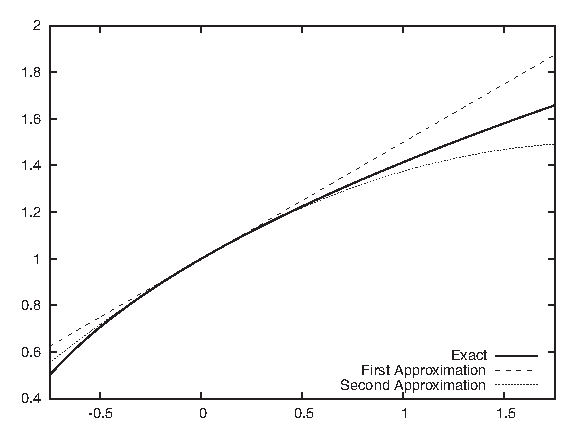
\includegraphics{img/perturb1}}
  \caption{The square-root function $\sqrt{1+x}$ and the first two 
    approximations around $x=0$.}
  \label{fig:perturb1}
\end{figure}

So far everything has been exact, but to make progress we need to make
an approximation. In this case, we replace the square root by a local
approximation around $1$. (Remember: $\epsilon$ is small,  and
$\sqrt{1}$ is easy.) Every smooth function can be replaced by a
straight line locally, and if we don't go too far, then that
approximation turns out to be quite good (see Figure
\ref{fig:perturb1}). These approximations can be derived in a
systematic fashion by a process known as \emph{Taylor expansion}. The
figure shows both the simplest approximation, which is just a straight
line, and also the next-higher (second-order) approximation, which is
even better.

Taylor expansions are so fundamental that they are almost considered a
\emph{fifth} basic operation (after addition, subtraction,
multiplication, and division). See Appendix \ref{app:calculus} for a
little more information on them.

With the linear approximation in place, our problem has now become
quite tractable:
%
\begin{align*}
\sqrt{17} & \approx 4 \left( 1 + \frac{\epsilon}{2} + \dotsb \right) \\
          & = 4 + 2 \epsilon
\end{align*}
%
We can now plug the numeric value $\epsilon = 1/16$ back in:
$\sqrt{17} \approx 4 + 2/16 = 4.125$. The exact value is $\sqrt{17} =
4.12310\dots$. Our approximation is pretty good.

% \soon{Second Example}

\subsection{Error Propagation}

Error propagation considers situations where we have some quantity $x$
and an associated uncertainty $\delta x$. We write $x \pm \delta x$ to
indicate that we expect the true value to lie anywhere in the range
from $x - \delta x$ to $x + \delta x$. In other words, we have not
just a single value for the quantity $x$, but instead a whole range of
possible values.

Now suppose we have several quantities---each with its own error
term---and we need to combine them in some fashion. We probably know
how to work with the quantities themselves, but what about the
uncertainties? For example, we know both the height and width of a
rectangle to within some range: $h+\delta h$ and $w+\delta w$. We also
know that the area is $A = h w$ (from basic geometry). But what can we
say about the uncertainty in the area?

This kind of scenario is ideal for the perturbative methods discussed
earlier: the uncertainties are ``small,'' so we can use simplifying
approximations to deduce their behavior.

Let's work through the area example:
%
\begin{align*}
A & = ( h \pm \delta h ) ( w \pm \delta w ) \\[4pt]
  & = h w \paren{1 \pm \frac{\delta h}{h}} 
          \paren{1 \pm \frac{\delta w}{w}} \\[4pt]
  & = h w \paren{1 \pm \frac{\delta h}{h} \pm \frac{\delta w}{w}
                   + \frac{\delta h}{h} \frac{\delta w}{w} }
\end{align*}
%
Here again we have factored the primary terms out, to end up with
terms of the form $1 + \text{\itshape small stuff}$, because that
makes life easier. This also means that, instead of expressing the
uncertainty through the \emph{absolute} error $\delta h$ or $\delta
w$, we express them through the \emph{relative} error $\delta h/h$ or
$\delta w/w$. (Observe that if $\delta h \ll h$, then $\delta h/h \ll
1$.)

So far, everything has been exact. Now comes the approximation: the
error terms are small (in fact, smaller than $1$); hence their product
is extra-small, and we can therefore drop it. Our final result is thus
$A = h w \paren{ 1 \pm ( \frac{\delta h}{h} + \frac{\delta w}{w} ) }$
or, in words: ``When multiplying two quantities, their relative errors
add.''  So if I know both the width and the height to within 10
percent each, then my uncertainty in the area will be 20 percent.

Here are a few more results of this form, which are useful whenever
you work with quantities that have associated uncertainties (you 
might want to try deriving some of these yourself):
\begin{align*}
( x \pm \delta x ) + ( y \pm \delta y ) 
  & = x + y \pm ( \delta x + \delta y ) 
  & \text{Sum} \\[4pt]
( x \pm \delta x ) \cdot ( y \pm \delta y ) 
  & = x y \paren{ 1 \pm \paren{ \frac{\delta x}{x} + \frac{\delta y}{y} }}
  & \text{Product} \\[4pt]
\frac{ x \pm \delta x }{ y \pm \delta y }
  & = \frac{x}{y} \paren{ 1 \pm \paren{ \frac{\delta x}{x} 
                                        + \frac{\delta y}{y} } }
  & \text{Fraction} \\[4pt]
\sqrt{x+\delta x} 
  & = \sqrt{x} \sqrt{1 + \frac{\delta x}{x} }
    \approx \sqrt{x} \paren{ 1 + \frac{1}{2} \frac{\delta x}{x} } 
  & \text{Square root} \\[4pt]
\log( x+\delta x)
  & = \log \paren{ x \paren{1 + \frac{\delta x}{x} } }
    \approx \log x + \frac{\delta x}{x}
  & \text{Logarithm}
\end{align*}

The most important ones are the first two: when adding (or
subtracting) two quantities, their absolute errors add; and when
multiplying (or dividing) two quantities, their relative errors add.
This implies that, if one of two quantities has a significantly larger
error than the other, then the larger error dominates the final
uncertainty.

Finally, you may have seen a different way to calculate errors that
gives slightly tighter bounds, but it is only appropriate if the
errors have been determined by calculating the variances in
\emph{repeated measurements} of the same quantity. Only in that case
are the statistical assumptions valid upon which this alternative
calculation is based.  For guesstimation, the simple (albeit more
pessimistic) approach described here is more appropriate.

% ============================================================
\section{Workshop: The Gnu Scientific Library (GSL)}

\index{guesstimation!GSL (Gnu Scientific Library)|(} 
\index{GSL (Gnu Scientific Library)|(} 
\index{Gnu Scientific Library (GSL)|(} 
\index{software!GSL|(}

What do you do when a calculation becomes too involved to do it in
your head or even on the back of an envelope? In particular, what can
you do if you \emph{need} the extra precision that a simple
order-of-magnitude estimation (as practiced in this chapter) will not
provide? Obviously, you reach for a numerical library!

The Gnu Scientific Library, or GSL, 
(\url{http://www.gnu.org/software/gsl/}) is the best currently available open
source library for numerical and scientific calculations that I am
aware of. The list of included features is comprehensive, and the
implementations are of high quality. Thanks to some unifying
conventions, the API, though forbidding at first, is actually quite
easy to learn and comfortable to use. Most importantly, the library is
mature, well documented, and reliable.

Let's use it to solve two rather different problems; this will give us
an opportunity to highlight some of the design choices incorporated
into the GSL.  The first example involves matrix and vector handling:
we will calculate the singular value decomposition (SVD) of a matrix.
The second example will demonstrate how the GSL handles non-linear,
iterative problems in numerical analysis as we find the minimum of a
nonlinear function.

The listing that follows should give you a flavor of what vector and
matrix operations look like when using the GSL. First, we allocate a
couple of (two-dimensional) vectors and assign values to their
elements. We then perform some basic vector operations: adding one
vector to another and performing a dot product. (The result of a dot
product is a scalar, not another vector.) Finally, we allocate and
initialize a matrix and calculate its SVD. (See Chapter
\ref{ch:reduction} for more information on vector and matrix
operations.)\vspace*{6pt}

\begin{verbatim}
/* Basic Linear Algebra using the GSL */

#include <stdio.h>
#include <gsl/gsl_vector.h>
#include <gsl/gsl_matrix.h>
#include <gsl/gsl_blas.h>
#include <gsl/gsl_linalg.h>

int main() \{
  double r;

  gsl_vector *a, *b, *s, *t;
  gsl_matrix *m, *v;


  /* --- Vectors --- */
  a = gsl_vector_alloc( 2 );    /* two dimensions */
  b = gsl_vector_alloc( 2 );

  /* a = [ 1.0, 2.0 ] */
  gsl_vector_set( a, 0, 1.0 ); 
  gsl_vector_set( a, 1, 2.0 );

\end{verbatim}
\begin{verbatim}
  /* a = [ 3.0, 6.0 ] */
  gsl_vector_set( b, 0, 3.0 );
  gsl_vector_set( b, 1, 6.0 );
 
  /* a += b (so that now a = [ 4.0, 8.0 ]) */
  gsl_vector_add( a, b );
  gsl_vector_fprintf( stdout, a, "%f" );

  /* r = a . b (dot product) */
  gsl_blas_ddot( a, b, &r );
\end{verbatim}\vspace*{-6pt}
\makeatletter
\def\texttt#1{{\fontsize{8}{10}\ttfamily\selectfont#1}}
\makeatother
\hspace*{26pt}\texttt{fprintf( stdout, "\%f$\backslash$n", r );}\vspace*{-6pt}
\begin{verbatim}

  /* --- Matrices --- */
  s = gsl_vector_alloc( 2 );
  t = gsl_vector_alloc( 2 ); 

  m = gsl_matrix_alloc( 2, 2 );
  v = gsl_matrix_alloc( 2, 2 );

  /* m = [ [1, 2], 
           [0, 3] ] */
  gsl_matrix_set( m, 0, 0, 1.0 );
  gsl_matrix_set( m, 0, 1, 2.0 );
  gsl_matrix_set( m, 1, 0, 0.0 );
  gsl_matrix_set( m, 1, 1, 3.0 );

  /* m = U s V^T (SVD : singular values are in vector s) */
  gsl_linalg_SV_decomp( m, v, s, t );
  gsl_vector_fprintf( stdout, s, "%f" );


  /* --- Cleanup --- */
  gsl_vector_free( a );
  gsl_vector_free( b );
  gsl_vector_free( s );
  gsl_vector_free( t );

  gsl_matrix_free( m );
  gsl_matrix_free( v );

  return 0;
\}
\end{verbatim}


It is becoming immediately (and a little painfully) clear that we are
dealing with plain C, not C++ or any other more modern,
object-oriented language! There is no operator overloading; we must
use regular functions to access individual vector and matrix elements.
There are no namespaces, so function names tend to be lengthy. And of
course there is no garbage collection!

What is \emph{not} so obvious is that element access is actually
boundary checked: if you try to access a vector element that does not 
exist (\eg, \texttt{gsl\_vector\_set( a, 4, 1.0 );}), then the~GSL
internal error handler will be invoked. By default, it will halt the
program and print a message to the screen.  This is\vadjust{\pagebreak} quite generally
true: if the library detects an error---including bad inputs, failure
to converge numerically, or an out-of-memory situation---it will
invoke its error handler to notify you. You can provide your own error
handler to respond to errors in a more flexible fashion.  For a fully
tested program, you can also turn range checking on vector and matrix
elements \emph{off} completely, to achieve the best possible runtime
performance.

Two more implementation details before leaving the linear algebra
example: although the matrix and vector elements are of type
\texttt{double} in this example, versions of all routines exist for
integer and complex data types as well. Furthermore, the GSL will use
an optimized implementation of the BLAS (Basic Linear Algebra
Subprograms) API if one is available; if not, the GSL comes with its
own, basic implementation.

Now let's take a look at the second example. Here we use the GSL to
find the minimum of a one-dimensional function. The function to
minimize is defined at the top of the listing: $x^2 \log(x)$. In
general, nonlinear problems such as this must be solved iteratively:
we start with a guess, then calculate a new trial solution based on
that guess, and so on until the result meets whatever stopping
criteria we care to define.

At least that's what the introductory textbooks tell you.

In the main part of the program, we instantiate a ``minimizer,'' which
is an encapsulation of a specific minimization algorithm (in this
case, Golden Section Search---others are available, too) and
initialize it with the function to minimize as well as our initial
guess for the interval containing the minimum.

Now comes the surprising part: an explicit loop! In this loop, the
``minimizer'' takes a single step in the iteration ({\it i.e.}, 
calculates a new, tighter interval bounding the minimum) but then
essentially hands control back to us. Why so complicated? Why can't we
just specify the desired accuracy of the interval and let the library
handle the entire iteration for us? The reason is that real problems
more often than not don't converge as obediently as the textbooks
suggest! Instead they can (and do) fail in a variety of ways: they
converge to the wrong solution, they attempt to access values for
which the function is not defined, they attempt to make steps that
(for reasons of the larger system of which the routine is only a small
part) are either too large or too small, or they diverge entirely.
Based on my experience, I have come to the conclusion that \emph{every
  nonlinear problem is different} (whereas every linear problem is the
same), and therefore generic black-box routines don't work!

This brings us back to the way this minimization routine is
implemented: the required iteration is not a black box and instead is
open and accessible to us. We can simply monitor its progress (as we
do in this example, by printing every iteration step to the screen),
but we could also interfere with it---for instance to enforce some
invariant that is specific to our problem. The ``minimizer'' does as
much as it can by calculating and proposing a new interval;
ultimately, however, we are in control over how the iteration
progresses. (For the textbook example used here, this doesn't matter,
but it makes all the difference when you are doing serious numerical
analysis on real problems!)\vspace*{9pt}

\begin{verbatim}
/* Minimizing a function with the GSL */

#include <stdio.h>
#include <gsl/gsl_min.h>

double fct( double x, void *params ) \{ 
  return x*x*log(x);
\}

int main() \{
  double a = 0.1, b = 1; /* interval which bounds the minimum */

  gsl_function f;        /* pointer to the function to minimize */
  gsl_min_fminimizer *s; /* pointer to the minimizer instance */
\end{verbatim}
\begin{verbatim}

  f.function = &fct;     /* the function to minimize */
  f.params = NULL;       /* no additional parameters needed */

  /* allocate the minimizer, choosing a particular algorithm */
  s = gsl_min_fminimizer_alloc( gsl_min_fminimizer_goldensection );

  /* initialize the minimizer with a function an an initial interval */
  gsl_min_fminimizer_set( s, &f, (a+b)/2.0, a, b );

  while ( b-a > 1.e-6 ) \{
    /* perform one minimization step */
    gsl_min_fminimizer_iterate( s );

    /* obtain the new bounding interval */
    a = gsl_min_fminimizer_x_lower( s );
    b = gsl_min_fminimizer_x_upper( s );

\end{verbatim}\vspace*{-9pt}
\hspace*{34pt}\texttt{printf( "\%f\t\%f$\backslash$n", a, b );}\vspace*{-6pt}
\begin{verbatim}
  \} 

\end{verbatim}\vspace*{-9pt}
\hspace*{26pt}\texttt{printf( "Minimum Position: \%f\t Value: \%f$\backslash$n",}\vspace*{-6pt}
\begin{verbatim}
          gsl_min_fminimizer_x_minimum(s), gsl_min_fminimizer_f_minimum(s) );

  gsl_min_fminimizer_free( s );

  return 0;
\}
\end{verbatim}


\makeatletter
\def\texttt#1{{\fontsize{8.5}{10}\ttfamily\selectfont#1}}
\makeatother

Obviously, we have only touched on the GSL. My primary intention in
this section was to give you a sense for the way the GSL is designed
and for what kinds of considerations it incorporates. The list of
features is extensive---consult the documentation for more
information.

\index{guesstimation!GSL (Gnu Scientific Library)|)} 
\index{GSL (Gnu Scientific Library)|)} 
\index{Gnu Scientific Library (GSL)|)} 
\index{software!GSL|)}

% ============================================================
\section{Further Reading}

\begin{itemize}
\item \cit{Guesstimation: Solving the World's Problems on the Back of
    a Cocktail Napkin}{Lawrence Weinstein and John A.\ Adam}{Princeton
    University Press}{2008}
  This little book contains about a hundred guesstimation problems
  (with solutions!) from all walks of life. If you are looking for
  ideas to get you started, look no further.

\item \citnobreak{Programming Pearls}{Jon Bentley}{2nd ed.,
    Addison-Wesley}{1999}; also, \cit{More Programming Pearls:
    Confessions of a Coder}{Jon Bentley}{Addison-Wesley}{1989}
  These two volumes of reprinted magazine columns are delightful to
  read, although (or because) they breathe the somewhat dated
  atmosphere of the old Bell Labs. Both volumes contain chapters on
  guesstimation problems in a programming context.

\item \cit{Back-of-the-Envelope Physics}{Clifford E.\ Swartz}{Johns
    Hopkins University Press}{2003}
  Physicists regard themselves as the inventors of back-of-the-envelope
  calculations. This book contains a set of examples from introductory
  physics (with solutions).

\item \cit{The Flying Circus of Physics}{Jearl Walker}{2nd ed.,
    Wiley}{2006} 
  If you'd like some hints on how to take an interest in the world
  around you, try this book. It contains hundreds of everyday
  observations and challenges you to provide an explanation for each.
  Why are dried coffee stains always darker around the rim?  Why are
  shower curtains pulled inward?  Remarkably, many of these
  observations are still not fully understood! (You might also want to
  check out the rather different and more challenging first edition.)

\item \cit{Pocket Ref}{Thomas J.\ Glover}{3rd ed., Sequoia
    Publishing}{2009}
  This small book is an extreme example of the ``lookup'' model. It
  seems to contain almost everything: strength of wood beams,
  electrical wiring charts, properties of materials, planetary data,
  first aid, military insignia, and sizing charts for clothing.  It
  also shows the limitations of an overcomplete collection of trivia:
  I simply don't find it all that useful, but it is interesting for
  the breadth of topics covered.

% The World almanac and book of facts

%\item \cit{One Hundred Essential Things You Didn't Know You Didn't
%     Know: Math Explains Your World}{John D.\ Barrow}{W.\ W.\ Norton \&
%     Company}{2009}
% 
% 
%\item \cit{Used Math For The First Two Years of College Science}{Clifford 
%     E.\ Swartz}{AAPT}{1993}
% 
%\item \cit{Surely You're Joking, Mr.\ Feynman! (Adventures of a
%     Curious Character)}{Richard P.\ Feynman and Ralph Leighton}{W.\ W.
%     Norton \& Co.}{1997}
\end{itemize}
